\documentclass[12pt,twoside]{report}
\usepackage[a4paper,width=150mm,top=25mm,bottom=25mm,bindingoffset=6mm]{geometry}
\usepackage[utf8]{inputenc}
\usepackage{graphicx}
\usepackage{fancyhdr}
\usepackage[acronym]{glossaries}
\graphicspath{ {images/} }
\usepackage[sorting=ynt,backend=biber]{biblatex}
% \usepackage{svg}
\usepackage[inkscapeformat=png]{svg}
\addbibresource{References.bib}

\includeonly{preliminary/title.tex,%
preliminary/dedication.tex,%
preliminary/abstract.tex,%
chapters/introduction.tex,%
chapters/chapter1.tex
}
\makeglossaries
% \newacronym{kgs}{KGs}{Knowledge Graphs}
% \newacronym{nlp}{NLP}{Natural Language Processing}
% \acro{ecu}[ECU]{European currency unit}
% \begin{acronym}[ECU]


% \chapter*{List of abbreviations} \label{LOA}
\begin{acronym}
\acro{kg}[KG]{Knowledge graph}
\acro{kb}[KB]{Knowledge base}
\acro{qe}[QE]{Questioning Engine}
\acro{nlp}[NLP]{Natural Language Processing}

\acro{qg}[QG]{Question generation}

\acro{ner}[NER]{Named Entity Recognition}
\acro{adp}[adp]{adposition}
\acro{pobj}[pobj]{prepositional object}
\acro{dobj}[dobj]{direct object}
\acro{nsubj}[nsubj]{nominal subject}
\acro{conj}[conj]{coordinating conjunction}
\acro{amod}[amod]{adjectival modifier}
\acro{POS}[POS]{part of speech}
\acro{pron}[pron]{pronoun}
\acro{SRO}[SRO]{subject,relation and object}
\acro{Tf-Idf}[Tf-Idf]{Term frequency-Inverse document frequency}
\acro{Tf}[Tf-Idf]{Term frequency}
\acro{Idf}[Idf]{Inverse document frequency}
\acro{KNN}[KNN]{\textit{k} -Nearest Neighbors}
\acro{RNN}[RNN]{Recurrent Neural Network}
\acro{ALL}[ALL]{Adaptive LogSoftmax with Loss}
\acro{NLLLoss}[NLLLoss]{Negative log likelihood loss}
\acro{BPTT}[BPTT]{Back Propagation through time}
\acro{DAG}[DAG]{directed acyclic graph }
\acro{SGD}[SGD]{Stochastic gradient descent }
\acro{CLR}[CLR]{Cyclic learning rate }
\acro{LTR}[LTR]{Learn to Rank }
\acro{IR}[IR]{Information Retrieval }
\acro{AI}[AI]{Artificial Intelligence }
\acro{PMF}[PMF]{Probability Mass Function }
\acro{MSE}[MSE]{Mean Squared Error}
\acro{GAN}[GAN]{generative adversarial network}
\acro{PIM}[PIM]{Product Information Management}
\acro{SKU}[SKU]{stock-keeping unit}

\acro{SEO}[SEO]{Search Engine Optimization}

\end{acronym}



\begin{document}

%--------------- Prelimanary pages -------------
\pagenumbering{roman}
\pagestyle{plain}

%--------------------------------------------
\begin{titlepage}

    \vspace*{3\baselineskip}
        \begin{flushright}        
  
                
\includegraphics[scale=0.3]{SRH_Hochschule_Heidelberg_logo.svg.png}
           
        \end{flushright}
    \vspace*{3\baselineskip}

    \centering
   


    {\Large \bfseries Application of Natural language processing in E-Commerce \\ Predicting product taxonomy}
    \vspace*{3\baselineskip}

    {\Large Master Thesis}
    \vspace*{1\baselineskip}

    {\Large by }
    \vspace*{2\baselineskip}

    {\Large  \bfseries Shoney Arickathil }
    \vspace*{0.5\baselineskip}

    {\Large  Student no: 11017678 }
    \vspace*{2\baselineskip}

    {\Large \today}
    \vspace*{8\baselineskip}

    % \includegraphics[width=0.35\linewidth]{srhlogo}

    {\Large  Masters in Applied Computer Science }
    \vspace*{0.5\baselineskip}

    {\Large  SRH University Heidelberg \\ School of Informatics}  
    \vspace*{6\baselineskip}

    \begin{minipage}{\textwidth}
        \begin{flushleft} % Left-align supervisor's name
            \large Primary Supervisor: \hfill \bfseries Prof. Dr. Gerd Moeckel
           
        \end{flushleft}
       
       
    \end{minipage}

    


   
    
\end{titlepage}

\include{preliminary/copyright.tex}
\chapter*{}

\begin{center}
    \vfill
    {\itshape Dedicated to my \ldots.}
    \vfill
\end{center}
\include{preliminary/approval-sheet.tex}

\begin{titlepage}
    \begin{flushright}
        
  
\section*{Certificate}
\justifying
This is to certify that the Project Report titled \textbf{Machine Learning for traffic flow prediction at different junctions}, submitted by \textbf{Cyril John Arickathil (M22RM210)} to the \textbf{Indian Institute of Technology Jodhpur} only for the award of the degree of \textbf{M.Tech in Robotics and Mobility Systems (RMS)} is a Bonafide record of the work under my supervision. To the best of my knowledge, the contents of this report, in full or in parts, have not been submitted to any other Institute or University for the award of any degree or diploma.
\vspace*{3\baselineskip}




{\large  \bfseries  Dr. Ranju Mohan }


\end{flushright}

\end{titlepage}


\begin{titlepage}
    \begin{flushright}
        
  
\section*{Acknowledgment}
\justifying
I would like to extend my deepest gratitude to \textbf{ Dr. Ranju Mohan} for her invaluable guidance
and support as my project supervisor. Her insightful feedback, unwavering encouragement, and
extensive knowledge have been instrumental in the successful completion of this project. Dr.
Mohan's dedication to excellence and her willingness to share her expertise have greatly
enhanced my learning experience. I am truly grateful for her mentorship and the opportunity
to work under her supervision. Her insights and expertise were crucial to the successful
completion of this work.

I am also immensely grateful to my examiners, \textbf{Dr. Bhupendra Singh} and Dr. Riby Abraham
Boby, for their thorough evaluation, constructive feedback, and suggestions, which greatly
contributed to the enhancement of this project.

My heartfelt thanks go to the program coordinators, \textbf{ Dr. Gourav Bhatnagar} and Dr. Dilpreet
Kaur, for their unwavering support, efficient coordination, and assistance in all administrative
matters, making this academic journey a smooth and enriching experience.
Finally, I would like to acknowledge the support and encouragement from my family,my elder brother, friends,
and colleagues, without whom this project would not have been possible.
\vspace*{3\baselineskip}


Thank you, \\

{\large  \bfseries Cyril John Arickathil }


\end{flushright}

\end{titlepage}


\chapter*{}

\begin{center}
    \vfill
    {\itshape Dedicated to my \ldots.}
    \vfill
\end{center}
\begin{abstract}
    

\begin{center}
    Shoney Arickathil, School of Informatics, SRH Hochschule Heidelberg \\

Master Thesis \\
\textbf{Application of Natural language processing in ECommerce}\\
\textbf{Predicting product taxonomy}

\end{center}


Electronic commerce started in early 1990's in which the business transactions are conducted through computer networks. The ease of buying a product online has reduced physical work and time required for decision-making by compare the product features. A wide range of products are sold online. One of the challenge is to well define a products' taxonomy. A product taxonomy is a hierarchical structure to organize the products in an E-commerce platform in such a way that customers can find the product in the fewest possible clicks.
Product taxonomy for the same product may differ based on the supplier and manufacturer (sources). Hence, product taxonomy details cannot be imported directly from the sources into the E-commerce platform. Product details cannot be live until its taxonomy is not well-defined, this delays the time of product availability for customers. 

In this thesis the author developed a machine learning classification model to predict the product taxonomy based on the features of the product. This is achieved with machine learning model. Experimenting and analyzing by varying  model's parameters facilitated to determine models performance.  

Initially, from the existing product taxonomy the features such as name and description were extracted. These extracted features were passed through process of text normalization, imputation of missing text to standardize it before converting it into One-Hot encoded format. These features and its lowest hierarchical level of category were processed by \acf*{RNN} machine learning model to learn the patterns of feature and classify it with the concept of probability distribution.

The result of predicting the lowest hierarchical level of product category based only on product name formed a foundation to create a machine learning model to predict the complete product taxonomy. As the level of category to be predicted increases the model's weight and product features need to be adjusted. 

\end{abstract}




\pagestyle{fancy}

\tableofcontents
\listoffigures
\listoftables


%----------------- chapters --------------------
\pagenumbering{arabic}

%---------------------------------------
\chapter{Introduction}

\section{Topic overview}


\chapter{Building a Knowledge graph} \label{sec:building-kg}

Graph-based knowledge representation has been researched for decades.
A \acf{kg} acquires and integrates information into an ontology and applies a reasoner to derive new knowledge \parencite{LisaEhrlinger}.
The knowledge base is a dataset with formal semantics that can contain different kinds of knowledge, for example, rules, facts, axioms, definitions, statements, and primitives \parencite{Davies.2008cop.2006}.

\begin{figure}[h!]
    \centering
    \includesvg[scale=0.5]{Thesis_kg.svg}
    \caption{\acl{kg} architecture}
    \label{fig:kg}
    \parencite[Chapter 4]{LisaEhrlinger}
\end{figure}

Figure \ref{fig:kg} illustrates the procsssing of plain text from various sources such as  Wikipedia API, PDF into a graph. This abstract architecture represented by \Citeauthor{LisaEhrlinger} of a \acl{kg} portraits the asumption that a \acl{kg} is more than a \acf{kb}. \acl{kg} is a combination of \acl{kb} and \acf{qe}. 

\Iac{qe} is a set of graph of possible questions that could be formed in reference to \iac{kb}. \acf{qg} for comprehensive reading is a challenging task. There are datasets available for  \acs{qg}, one of it is Stanford Question Answering Dataset v1.0 (SQuAD) consisting of questions posed by crowdworkers on a set of Wikipedia articles \parencite{PranavRajpurkar.}. The limitation with such a data set is that these do not contain unanserable questions. Building a machine learning model when no answer is supported was out of scope of SQuAD objective \parencite{LupeHernandez}.  Study on automatic question generation from an attention-based sequence learning model for  \ac{qg} and investigate the effect of encoding sentence- vs. paragraph-level information \parencite{DuXinya.29042017}, reduces reliance on handcrafted rule based systems.

\clearpage

\section{Fetching text corpus}


One of the first things required for \acf*{nlp} tasks is a creating a text corpus.
In linguistics and \acs{nlp}, corpus refers to a collection of texts. One of the objective of this paper is to web crawl and extract data related to "Motor Oil". Our intention is to fetch the unstructred text corpus specifically related to "Motor Oil" and to create a graph-based knowledge. 

Wikipedia\footnote{https://www.wikipedia.org/} is primarily an encyclopedia with the additional benefit of heavy linking between articles and without the size constraints of paper articles \parencite{TorstenZesch}. Wikipedia API \footnote{https://pypi.org/project/Wikipedia-API/}

\section{spaCy - Dependency Parsing} \label{dependencyparsing}

spaCy \parencite{spacy2} features neural models for parsing and entity recognition. These models can be trained for \acf{ner} , tagging and parsing. Its official page on usage\footnote {https://v2.spacy.io/usage/} provides in-depth code example for information extraction.

In figure \ref{fig:dp}, we see a complex sentence's dependency parsing. It has a \acf{nsubj}, connecting \acfp{pobj} with \acfp{adp} and no \acf{dobj}.

\begin{figure}[htp!]
    \centering    
    \includesvg[scale=0.16]{dependency-parser.svg}
    \caption{Navigating the parse tree and subtrees}
    \label{fig:dp}
\end{figure}

The \acs{nsubj} "oil", itself does not give a complete meaning. However, upon combining its dependency noun "Motor", which is "Motor oil"  gives us an understanding of the topic. Traversing from \acs{nsubj} to  \acfp{conj} provides us with three related compound nouns belonging to a similar group.

"Motor oil", "Engine Oil", "Engine Lubricant"

Traversing further right of the dependency tree we can extract the \acsp{pobj}.  An \acf{amod} "internal" is connecting compound noun "combustion engine".

\section{Knowledge graph with Networkx}

The directed graphs created with Networkx \parencite{hagberg2008exploring} is suitable for representing depedency parsing of a sentence mentioned in section \ref{dependencyparsing}. A knowledge base are represented as triples of \acf{SRO}. In which the subject and object are nodes or entities of a graph and relation are directed edges or links between the nodes.

\subsection{What to use as nodes n(x) and edges e(y)?}

In table \ref{table:1}, distigution of triples by  \acs{POS} tags is depicted. 
\begin{table}[h!]
\begin{center}
\begin{tabular}{>{$}l<{$} l}

triples   &   \acf{POS} tags   \\
\hline
n(subject)   &   \acs{nsubj} , \acs{pron}                          \\
n(object)  &   \acs{dobj}    , \acs{pobj}                     \\
e(relation)  &   \acs{adp}, verb
\end{tabular}
\end{center}
\caption{\acs{SRO} and \acs{POS} tags mappings}
\label{table:1}
\end{table}

\section{Summary}


In this chapter, using the dependency parsing of an unstructured sentence, building a knowledge graph is proposed.  The process involves textual information on a product from various sources pass through various methods such as dependency parsing, part of speech tagging, named entity relationship mapping. The processed text is created into a directed graph along with the question engine is called the knowledge graph.  

Further research has to be conducted on generating knowledge graph. As per \parencite{LisaEhrlinger}, there are limitations with knowledge graphs as comprehensive reading is a challenging task.

\appendix


\begin{appendices}

\chapter*{Appendices}
\addcontentsline{toc}{chapter}{Appendices}
% Additional appendices can be added here
\section{List of Abbreviations}
% \newacronym{kgs}{KGs}{Knowledge Graphs}
% \newacronym{nlp}{NLP}{Natural Language Processing}
% \acro{ecu}[ECU]{European currency unit}
% \begin{acronym}[ECU]


% \chapter*{List of abbreviations} \label{LOA}
\begin{acronym}
\acro{kg}[KG]{Knowledge graph}
\acro{kb}[KB]{Knowledge base}
\acro{qe}[QE]{Questioning Engine}
\acro{nlp}[NLP]{Natural Language Processing}

\acro{qg}[QG]{Question generation}

\acro{ner}[NER]{Named Entity Recognition}
\acro{adp}[adp]{adposition}
\acro{pobj}[pobj]{prepositional object}
\acro{dobj}[dobj]{direct object}
\acro{nsubj}[nsubj]{nominal subject}
\acro{conj}[conj]{coordinating conjunction}
\acro{amod}[amod]{adjectival modifier}
\acro{POS}[POS]{part of speech}
\acro{pron}[pron]{pronoun}
\acro{SRO}[SRO]{subject,relation and object}
\acro{Tf-Idf}[Tf-Idf]{Term frequency-Inverse document frequency}
\acro{Tf}[Tf-Idf]{Term frequency}
\acro{Idf}[Idf]{Inverse document frequency}
\acro{KNN}[KNN]{\textit{k} -Nearest Neighbors}
\acro{RNN}[RNN]{Recurrent Neural Network}
\acro{ALL}[ALL]{Adaptive LogSoftmax with Loss}
\acro{NLLLoss}[NLLLoss]{Negative log likelihood loss}
\acro{BPTT}[BPTT]{Back Propagation through time}
\acro{DAG}[DAG]{directed acyclic graph }
\acro{SGD}[SGD]{Stochastic gradient descent }
\acro{CLR}[CLR]{Cyclic learning rate }
\acro{LTR}[LTR]{Learn to Rank }
\acro{IR}[IR]{Information Retrieval }
\acro{AI}[AI]{Artificial Intelligence }
\acro{PMF}[PMF]{Probability Mass Function }
\acro{MSE}[MSE]{Mean Squared Error}
\acro{GAN}[GAN]{generative adversarial network}
\acro{PIM}[PIM]{Product Information Management}
\acro{SKU}[SKU]{stock-keeping unit}

\acro{SEO}[SEO]{Search Engine Optimization}

\end{acronym}


\section{Appendix A}
For this project, python client elasticsearch 6.8.2 is installed as the client needs to be compatible with Elastic search version being used. The official Python client provides mapping with Elasticsearch REST APIs.

\begin{lstlisting}[language=Python,caption={Elastic search},label={code:es_search}]
    resp=self.es.search("english-name-category",{"_source":["id","name","category"],
    'from':_from,
    'size' :_size ,
    "query": {"match_all": {}}})
    \end{lstlisting}
% Content for Appendix A goes here...

\subsection*{Confusion matrix}
\begin{lstlisting}[language=Python,caption={Confusion matrix},label={code:confusion matrix}]
def confusionMatix(self,df_en):
# Keep track of correct guesses in a confusion matrix
data = Data(df_en)
n_categories = len(data.all_category)

batch = random.choices(data.all_category,k=20)

confusion = torch.zeros(n_categories, n_categories)
n_confusion = 10000

# Go through a bunch of examples and record which are correctly guessed
for i in range(n_confusion):
    category, name, category_tensor, name_tensor = data.randomTrainingExample()
    if category in batch:
        output = self.evaluate(name_tensor)
        guess, guess_i = data.categoryFromOutput(output)
        category_i =data.all_category.index(category)
        confusion[category_i][guess_i] += 1

# Normalize by dividing every row by its sum
for i in range(20):
    confusion[i] = confusion[i] / confusion[i].sum()


# Set up plot
fig = plt.figure()
ax = fig.add_subplot(111)
cax = ax.matshow(confusion.numpy())
fig.colorbar(cax)

# Set up axes
ax.set_xticklabels([''] + data.all_category, rotation=45)
ax.set_yticklabels([''] + data.all_category)

# Force label at every tick
ax.xaxis.set_major_locator(ticker.MultipleLocator(1))
ax.yaxis.set_major_locator(ticker.MultipleLocator(1))

# sphinx_gallery_thumbnail_number = 2
plt.show()
plt.savefig('confusion.png', dpi=400)

\end{lstlisting}

\subsection*{Load PyTorch model}
\begin{lstlisting}[language=Python,caption={Load PyTorch model},label={code:Loadpt}]
class Predict():
    def __init__(self):
         self.rnn = torch.load('ngram-rnn-classification.pt')
        \end{lstlisting}
\clearpage
\section{Appendix B}
\begin{figure}[H]
    \centering    
    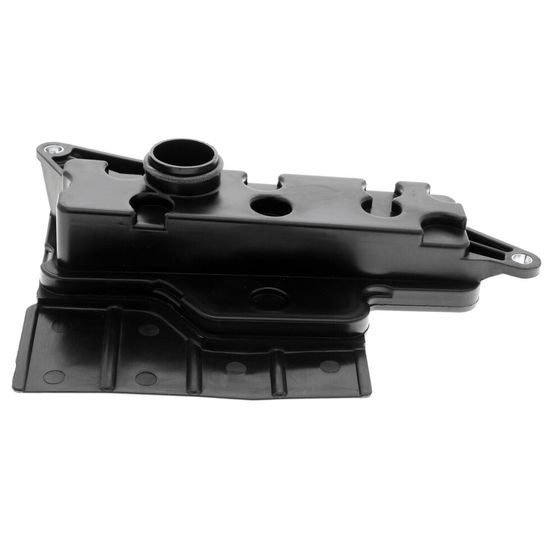
\includegraphics[scale=0.5]{ht_rm.jpg}
    \caption{Hydraulic filter automatic transmission VAICO V70-0613 for Lexus RX \parencite{RM}}
    \label{fig:sparepart}
\end{figure}

\end{appendices}


\clearpage
% \printglossary[type=\acronymtype]

% \printglossary

\printbibliography

\end{document}